%%%% CAPÍTULO 2 - REVISÃO DA LITERATURA (OU REVISÃO BIBLIOGRÁFICA, ESTADO DA ARTE, ESTADO DO CONHECIMENTO)
%%
%% O autor deve registrar seu conhecimento sobre a literatura básica do assunto, discutindo e comentando a informação já publicada.
%% A revisão deve ser apresentada, preferencialmente, em ordem cronológica e por blocos de assunto, procurando mostrar a evolução do tema.
%% Título e rótulo de capítulo (rótulos não devem conter caracteres especiais, acentuados ou cedilha)
\chapter{Fundamentação te\'orica}\label{cap:referencialTeorico}

Neste capítulo são apresentados alguns dos conceitos importantes para o entendimento
do trabalho. Sendo abordados assuntos como biometria, processamento de imagens, aprendizado 
profundo e reconhecimento facial.

\section{Microcontrolador}\label{sec:microcontrolador}

Um microcontrolador é um computador em um único \textit{chip} que incorpora um processador, 
memória, periféricos de entrada e saída, temporizadores e dispositivos de 
comunicação serial. Eles surgiram como uma evolução natural dos circuitos digitais 
devido à crescente complexidade. Chegou um ponto em que foi mais prático e 
econômico substituir a lógica das portas digitais por um conjunto de 
processador e \textit{software} \cite{penido2013}.

O primeiro microcontrolador, o "8048", foi lançado pela Intel em 1977 e evoluiu 
para a família "8051". Esses \textit{chips} são programados em linguagem \textit{Assembly} e 
possuem um conjunto de instruções poderoso \cite{penido2013}.

Atualmente, quando se trata de microcontrolador, uma boa opção é o ESP32 (\autoref{fig:esp32}). Mesmo não 
sendo o modelo mais potente, nem o mais compacto, ainda assim, possui um ótimo custo 
beneficio. Considerando sua simplicidade, poder de processamento e baixo consumo 
de corrente \cite{espressif2022c}.

\begin{figure}[h!]
    \centering
    \caption{ESP32-DevKitC.}
    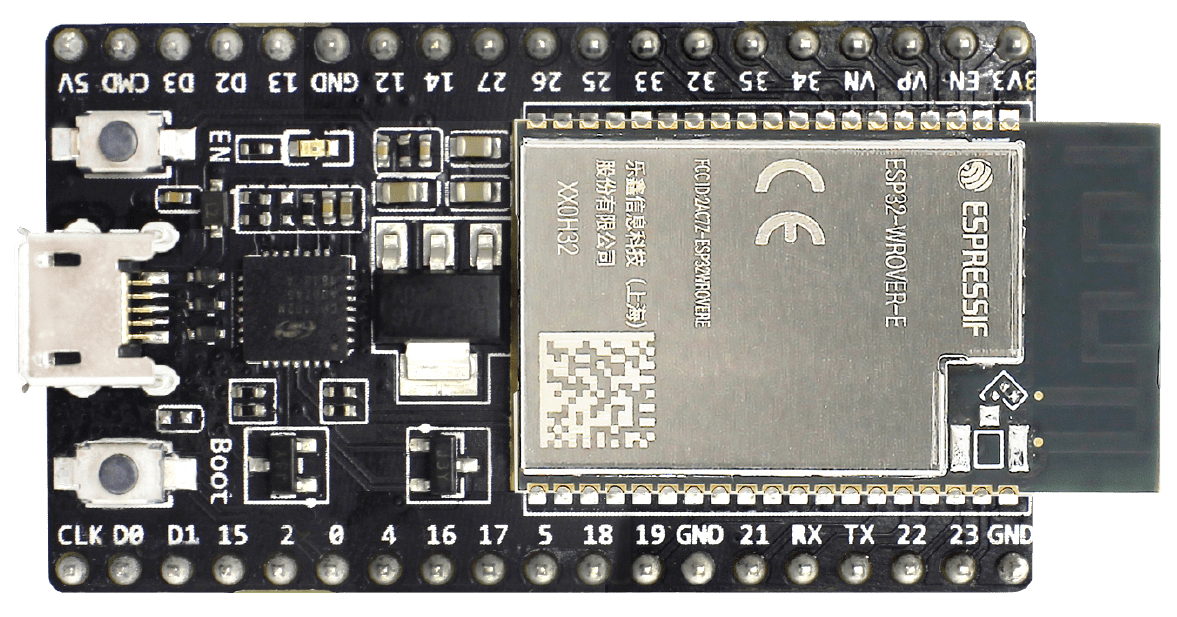
\includegraphics[scale=0.13]{figuras/esp323.png} 
    \legend{Fonte: Adaptado de \citeonline{espressifimg}.}
    \label{fig:esp32}
    \centering
\end{figure}

A versão escolhida para este projeto será o ESP32-CAM, onde além de possuir um 
\textit{chip} ESP32 integrado, nele também está incluso uma câmera, uma entrada para 
cartão SD e LED de alto brilho.

\subsection{PlatformIO}\label{sec:espacamento}

Uma forma para programar o ESP32 é utilizando o Arduino IDE. Um aplicativo de 
código aberto, escrito em C e C++, que permite a comunicação e gravação em \textit{chips} 
ATmega da família AVR. Entretanto, para gravar em \textit{chips} ESP32, basta ativar 
o utilitário Esptool.

Além do ambiente de desenvolvimento, outra vantagem é que o Arduino IDE 
possui inúmeras bibliotecas e documentação. Facilitando e assegurando o 
desenvolvimento de novos códigos, pois essas bibliotecas são constantemente 
testadas e atualizadas pela comunidade da plataforma Arduino.

\section{ESP-DL}\label{sec:formatacaoTexto}

ESP-DL é uma biblioteca de alto desempenho dedicada ao ESP32, ESP32-S2, 
ESP32-S3 e ESP32-C3, projetada para recursos de aprendizagem profunda. 

O \citeonline{espdl} oferece APIs para tarefas como inferência de redes 
neurais (NN), processamento de imagens, operações matemáticas e inclui 
alguns modelos de aprendizado profundo. Com essa biblioteca, você 
pode aproveitar os SoCs (System-on-Chip) da \textit{Espressif} de forma simples 
e ágil para implementar diversos tipo de aplicações.

\section{PROCESSAMENTO DE IMAGENS}\label{sec:processamento}

As técnicas de processamento de imagens começaram a surgir no final da década de 1960, 
para serem utilizadas no realce e restauração de imagens capturadas do espaço, 
como por exemplo, as imagens da missão Apollo. Logo em seguida essa tecnologia 
começou a ser empregada para processar imagens em diagnósticos médicos, e com 
o aumento de poder de processamento dos computadores, essas técnicas agora 
são empregadas nas mais diversas áreas de conhecimento \cite{gonzalez2010}.

Em processamento de imagens um conceito bastante utilizado é a binarização de
imagens, que consiste em duas classes distintas, o fundo e o objeto, esse processo 
serve para de certa forma separar ambas as classes.

Sendo assim, a forma mais simples de processamentos consiste na
bipartição do histograma, dando valores iguais a 0 (branco) aos pixels que estiverem
abaixo do valor de \textit{threshold} (T), e iguais a 255 (preto) aos pixels que estiverem 
acima desse valor. A \autoref{fig:escalacinza} mostra uma escala de tons 
de cinza, e a \autoref{fig:escalabinarizada} mostra essa mesma escala após passar 
por esse processamento, exemplificando o processo de binarização.

\begin{figure}[h!]
    \centering
    \caption{Escala de cinza}
    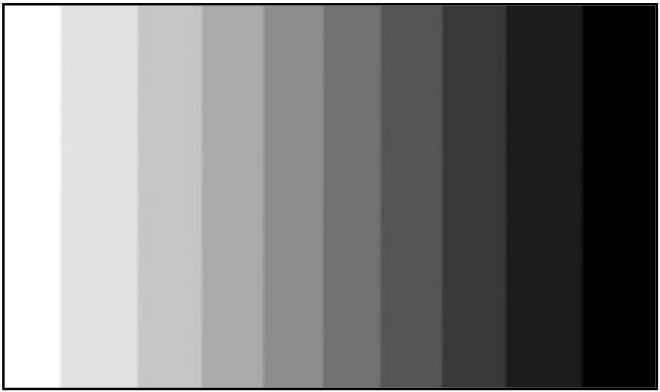
\includegraphics[scale=0.25]{figuras/escala_cinza.png} 
    \fonte{}%% Fonte
    \label{fig:escalacinza}
    \centering
\end{figure}

\begin{figure}[h!]
    \centering
    \caption{Escala de cinza binarizada}
    
\includegraphics[scale=0.25]{figuras/escala_binarizada.png} 
    \fonte{}%% Fonte
    \label{fig:escalabinarizada}
    \centering
\end{figure}

Especialmente durante o processo de reconhecimento de objetos. 
A segmentação é uma ferramenta indispensável para fins de análise e interpretação.

A segmentação de uma imagem é um procedimento importante no que tange
essas análises, uma vez que ela subdivide uma imagem em regiões que
posteriormente serão ou não tidas como de interesse, o que pode variar muito de
acordo com a aplicação \cite{gonzalez2010}.

Os principais algoritmos de segmentação se baseiam nas técnicas de
descontinuidade e similaridade, a abordagem de descontinuidade consiste em dividir
uma imagem com base nas mudanças bruscas mudanças de intensidade, como
ocorre nas bordas. Enquanto na técnica por similaridade a divisão da imagem
acontece por regiões que sejam semelhantes de acordo com um conjunto de critérios
preestabelecidos \cite{gonzalez2010}.

Por fim, uma outra técnica conhecida como esqueletização, 
consiste na representação de um conjunto de pontos no interior de um 
objeto de uma imagem. O esqueleto de uma região pode
ser definido pela transformada do eixo médio (MAT) do inglês (\textit{medial axis
transformation}). Nessa técnica são selecionados os elementos centrais de um objeto,
criando literalmente um esqueleto da imagem. MAT de uma região \textit{R} com uma borda
\textit{B} é definida como: para cada ponto \textit{p} contido na região, encontramos seu vizinho
mais próximo em \textit{B} (borda), e se houver mais de um vizinho então o ponto pertence
ao eixo médio, ou seja ao esqueleto \cite{gonzalez2010}.

O que pode ser visualizado com mais facilidade na \autoref{fig:esqueletizacao}:

\begin{figure}[h!]
    \centering
    \caption{Processo de esqueletização}
    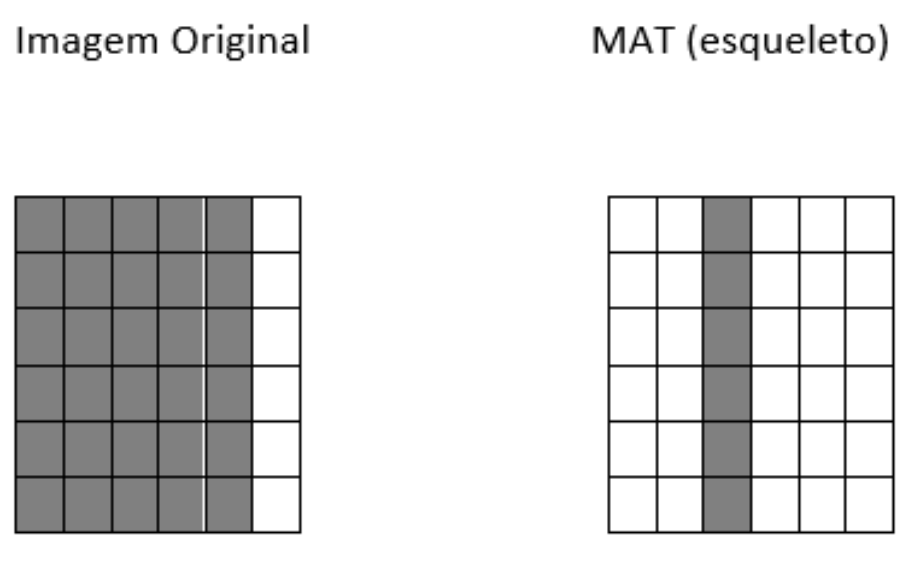
\includegraphics[scale=0.25]{figuras/esqueletizacao.png} 
    \fonte{}%% Fonte
    \label{fig:esqueletizacao}
    \centering
\end{figure}

\section{BIOMETRIA}\label{sec:biometria}

Com o avanço da tecnologia, hoje é possível realizar transações e pagamentos a 
partir de qualquer lugar, ou até mesmo, sem sair de casa, apenas com o uso de 
um dispositivo conectado a internet. Entretanto, também tornaram-se indispensáveis 
o uso de mecanismos de segurança, principalmente os que são capazes de identificar 
e comprovar quem realmente está utilizando esses serviços.

Por mais que existam outros processos de identificação, como por exemplo, cartões 
magnéticos, senhas, tags, etc., atualmente o processo considerado mais seguro é 
o baseado em biometria.

A biometria pode ser definida como o processo de identificação 
dos seres vivos. No intuito de distinguir os indivíduos, a partir de suas 
características únicas. É uma técnica que foi utilizada até mesmo pelos egípcios 
para o processo de identificação, baseando-se em características da
aparência dos indivíduos, como cor dos olhos e cicatrizes \cite{santos2007}.

\section{TIPOS DE BIOMETRIA}\label{sec:tiposBiometria}

De acordo com \citeonline{morais2010}, os principais tipos de biometria são:

\begin{itemize}
    \item Orelhas: Usa a anatomia da orelha para identificar indivíduos, abordagens 
    incomuns. Os pontos fortes são aceitabilidade e permanência; fraquezas, 
    singularidade e desempenho.

    \item Termograma da face e das mãos: O padrão de calor emitido pelo corpo 
    humano é uma característica de cada pessoa e pode ser captado por 
    infravermelho. Sistemas baseados em imagens termográficas não requerem 
    contato ou cooperação individual. No entanto, a captura de imagem continua 
    sendo um desafio em ambientes não controlados, pois é afetada por fontes de 
    calor que possivelmente podem estar próximas ao indivíduo. Seus pontos fortes 
    são a universalidade, a impostura e a singularidade.

    \item Impressão digital: recurso mais comumente usado em credenciais 
     automatizadas em grande escala.  Sua popularidade se deve em parte a 
     dispositivos de coleta de baixo custo e desempenho de processo razoável. 
     Embora a impressão digital não se modifique naturalmente ao longo dos anos, 
     ela é sensível aos fatores ambientais aos quais os indivíduos estão 
     submetidos, o que pode levar à sua alteração e deterioração. Trabalhadores 
     manuais, por exemplo, podem ver suas impressões digitais constantemente 
     alteradas devido a cortes profundos ou outros cortes em seus dedos.

    \item Íris: Formada durante o desenvolvimento fetal, estabiliza-se durante 
    os dois primeiros anos de vida. Sua textura é extremamente complexa e 
    fornece informações a serem utilizadas no reconhecimento facial. Tem um baixo grau 
    de impostura, pois é difícil até cirurgicamente alterar a textura da íris. 
    Seu ponto fraco está em sua capacidade de recuperação, requer equipamentos 
    caros e complexos, bem como cooperação individual.

    \item Voz: União de biometria comportamental e fisiológica. Ele não muda 
    em curtos períodos de tempo, mas é afetado por fatores como um simples frio, 
    estado emocional e ruído de fundo. Possui baixa exclusividade e não é 
    recomendado para identificação em larga escala. O ponto forte é a capacidade 
    de coleta e aceitabilidade, além do baixo custo dos coletores. Geralmente 
    indicado para verificação de identidade em conversas.
\end{itemize}

\section{RECONHECIMENTO FACIAL}\label{sec:reconhecimento}

Desde a infância, o ser humano adquire e desenvolve sua capacidade de reconhecer traços faciais, 
que é uma particularidade da visão e fundamental para relações sociais \cite{rouhani2019}.

Existem estudos sobre automatização do reconhecimento facial desde os anos 60. Os projetos iniciais nessa 
área dependiam do administrador encontrar manualmente as características faciais nas imagens, só 
então o sistema calculava as distâncias entre elas e comparava suas dimensões normalizadas com 
as referenciadas.

O processo de reconhecimento facial pode ser descrito a partir de uma imagem ou vídeo estático, 
identificando um ou múltiplos indivíduos a partir de um banco de dados de rostos previamente 
cadastrados. Assim, existem três abordagens conhecidas para reconhecimento:

\begin{itemize}
    \item Imagem a imagem: a amostra e a base de dados composta por imagens estáticas;

    \item Vídeo para vídeo: a amostra e o banco de dados que consiste em vídeos;

    \item Imagem para vídeo: o exemplo é um vídeo. O vídeo é comparado a um banco de 
    dados de imagens estáticas. Para esse caso, a biblioteca OpenCV possibilita,
     a partir da versão 2.4, o uso da classe FaceRecognizer para reconhecimento 
     facial. Os algoritmos atualmente disponíveis na biblioteca são: Fisherfaces 
     e Histogramas de Padrões Binários Locais (LBP).
\end{itemize}

Após a imagem ter sido lida e transformada em uma matriz da OpenCV, a mesma é
duplicada e redimensionada proporcionalmente para uma altura fixa. A imagem original 
é mantida para ser utilizada posteriormente. Em seguida a imagem é convertida para 
escalas de cinza e então equalizada para realçar o contraste e facilitar a detecção de faces.

A seguir, é feita a detecção das faces utilizando o classificador LBP
fornecido pela biblioteca OpenCV. Removendo o fundo ao redor da face, pois 
pode atrapalhar os algoritmos de reconhecimento.

As abordagens mais populares usadas no problema de reconhecimento facial são 
baseadas na localização e análise de atributos faciais como olhos, nariz e boca (\autoref{fig:haarcascate}), 
ou em análise global destes.

\begin{figure}[h!]
    \centering
    \caption{Reconhecimento baseado na localização dos olhos e nariz}
    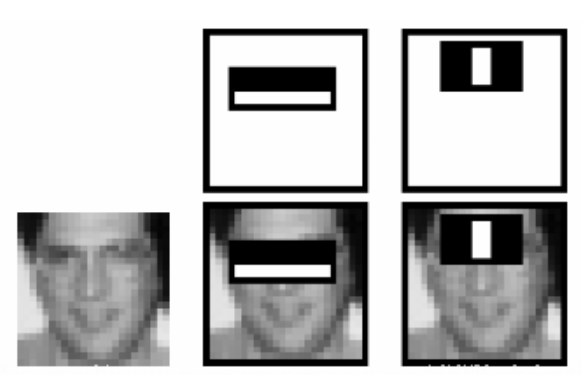
\includegraphics[scale=0.25]{figuras/haarcascate.png}
    \legend{Fonte: Adaptado de \citeonline{viola2004}.}
    \label{fig:haarcascate}
    \centering
\end{figure}

E com a comparação das informações extraídas com as informações
conhecidas, juntamente com uma pequena análise estatística, pode-se categorizar o
objeto e ainda determinar com precisão do que se trata \cite{gonzalez2010}.

\section{BIOMETRIA FACIAL PARA CONTROLE E ACESSO}\label{sec:biometriaFacial}

Os sistemas de identificação baseados em biometria são essencialmente sistemas de 
reconhecimento que, dadas informações biométricas, são capazes de distinguir padrões e 
classificá-los em diferentes classes ou categorias. \cite{morais2010}.

Ainda de acordo com o autor, algumas das principais características anatômicas, 
fisiológicas e comportamentais utilizadas em sistemas biométricos incluem 
impressão digital, impressão da mão, aparência facial, temperatura da face, 
retina, voz, assinatura, entre outras.

A biometria facial é o recurso biométrico mais utilizado por humanos para identificação 
pessoal. Embora usar a face para identificar conhecidos seja uma tarefa trivial para 
o ser humano, no entanto, é uma tarefa bastante complexa para computadores. Mesmo 
tendo um desempenho razoável em sistemas comerciais, um sistema biométrico facial 
impõem algumas restrições no fundo, como iluminação e o ângulo das imagens utilizadas.

Segundo \citeonline{cavalcanti2005}, alterações estéticas, como cabelo e barba, uso de
acessórios, como óculos e bonés, são fatores que aumentam as chances de falha no processo
de reconhecimento facial.

Para utilizar a face em sistemas biométricos é preciso seguir três
etapas fundamentais. São elas:

\begin{itemize}
    \item Detecção Facial: Responsável por definir e localizar uma ou mais
    faces;

    \item Extração de Características: Esta fase é responsável por remover o excesso de
    informações que rodeiam as faces detectadas, assim como selecionar as melhores
    características para serem utilizadas na próxima etapa;

    \item Reconhecimento Facial: Esta fase compara as características selecionadas pela fase
    anterior com outras previamente cadastradas em um banco de dados. Sendo
    responsável por encontrar um registro que se assemelhe ao que precisa ser
    identificado;

\end{itemize}